\documentclass{standalone}
\usepackage{tikz}
\usetikzlibrary{patterns, positioning}
\usetikzlibrary{shapes.misc}
\usepackage[outline]{contour}
\contourlength{1.5pt} 
\usepackage[sfdefault]{ClearSans} %% option 'sfdefault' activates Clear Sans as the default text font
\usepackage[T1]{fontenc}

\begin{document}
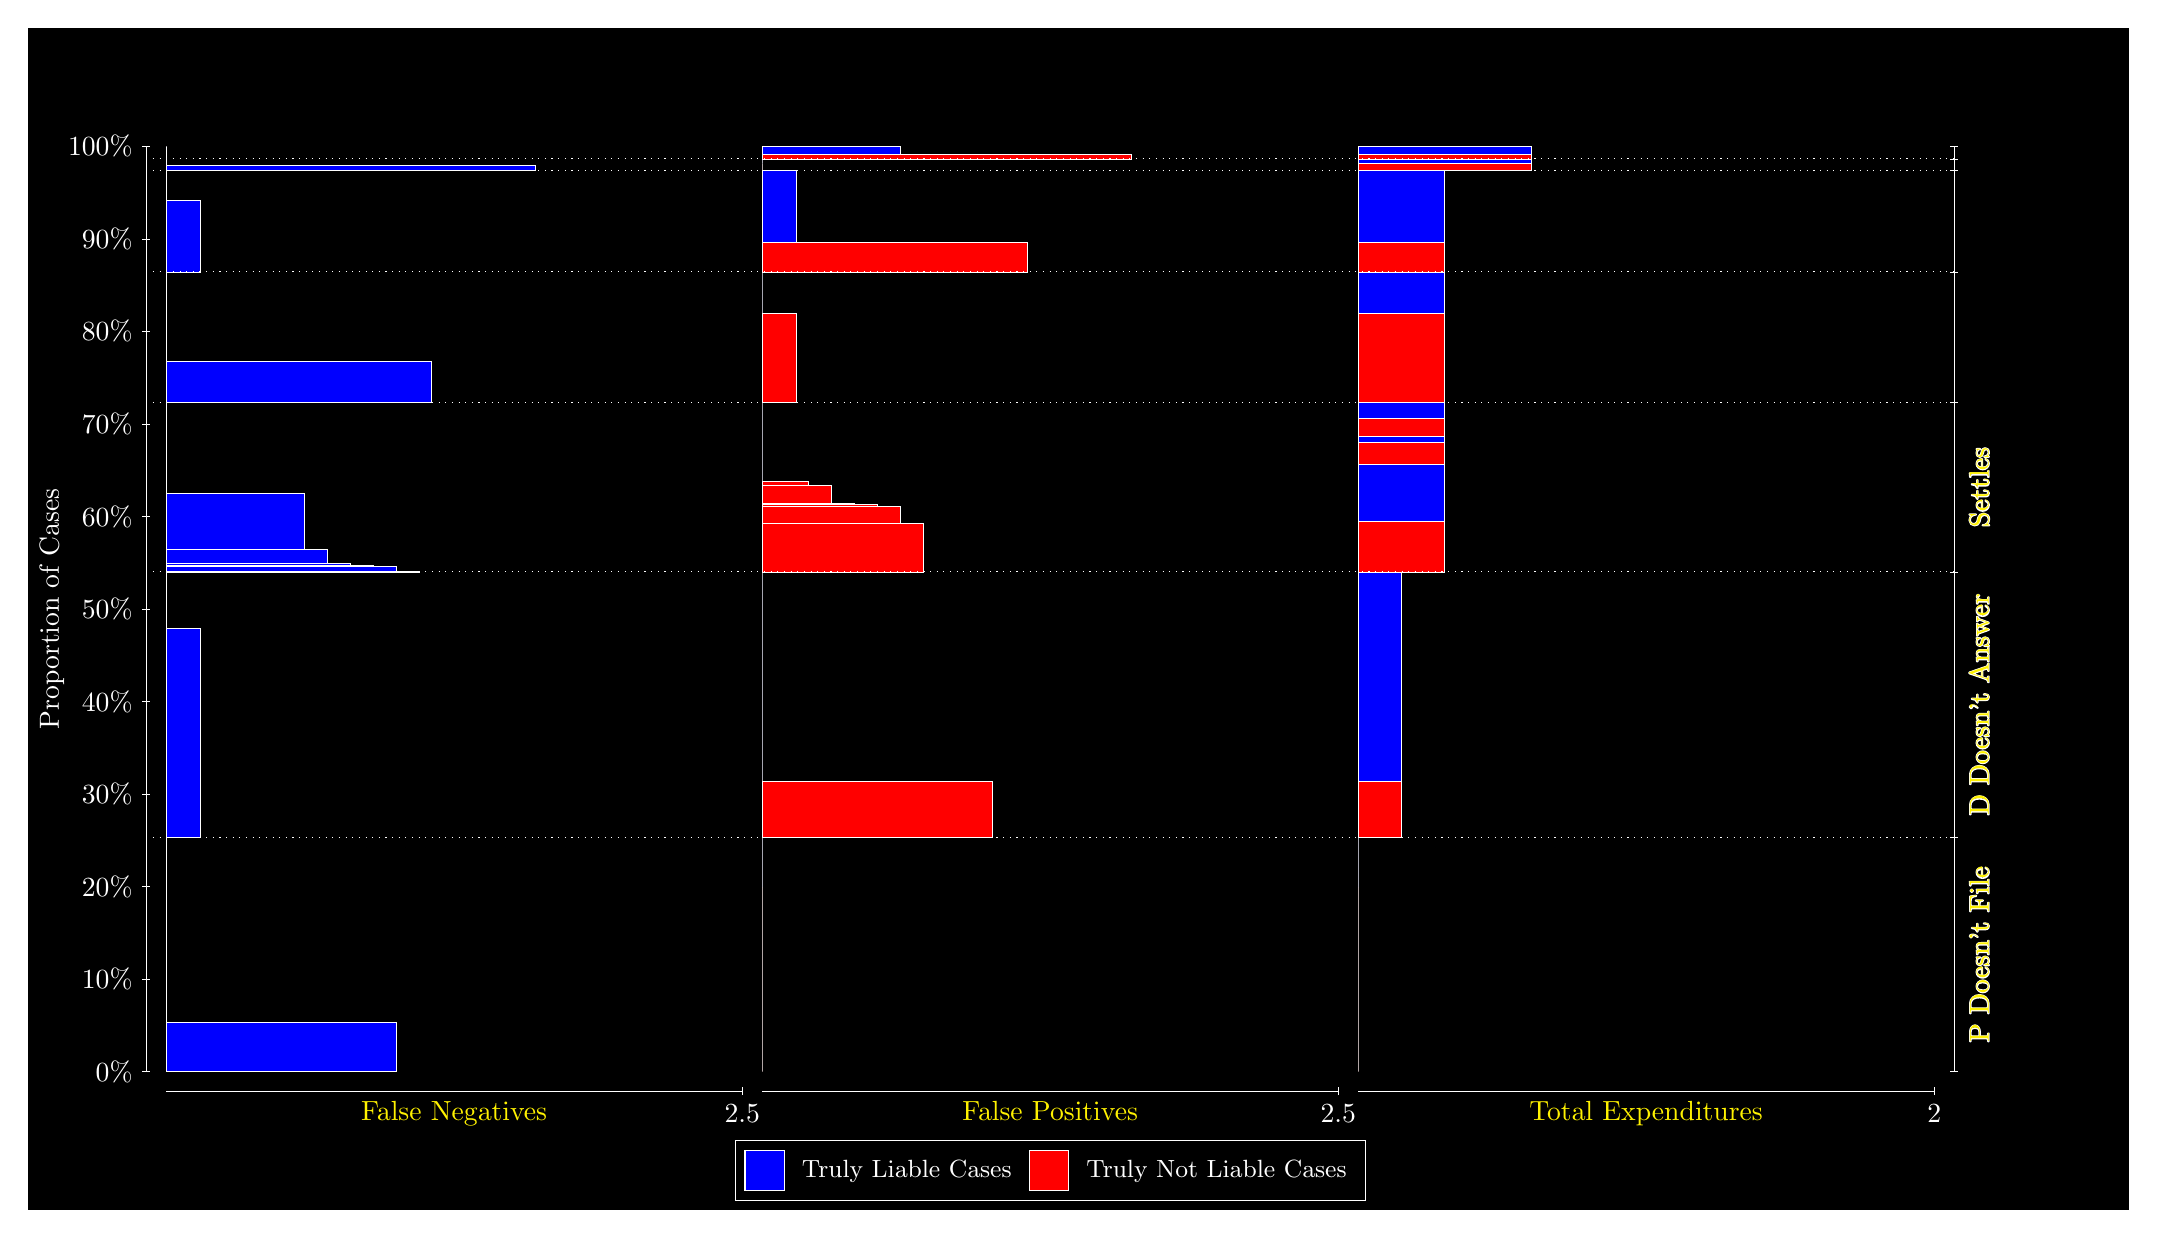
\begin{tikzpicture}
\draw[fill=black] (0,0) rectangle (26.667,15);
\draw[white, very thin] (1.5,1.75) -- (1.5,13.5);
\node[rotate=90, text=white, anchor=center] at (0.3, 7.625) {Proportion of Cases};
\draw[white, very thin] (1.45,1.75) -- (1.55,1.75);
\node[text=white, anchor=east] at (1.45, 1.75) {0\%};
\draw[white, very thin] (1.45,2.925) -- (1.55,2.925);
\node[text=white, anchor=east] at (1.45, 2.925) {10\%};
\draw[white, very thin] (1.45,4.1) -- (1.55,4.1);
\node[text=white, anchor=east] at (1.45, 4.1) {20\%};
\draw[white, very thin] (1.45,5.275) -- (1.55,5.275);
\node[text=white, anchor=east] at (1.45, 5.275) {30\%};
\draw[white, very thin] (1.45,6.45) -- (1.55,6.45);
\node[text=white, anchor=east] at (1.45, 6.45) {40\%};
\draw[white, very thin] (1.45,7.625) -- (1.55,7.625);
\node[text=white, anchor=east] at (1.45, 7.625) {50\%};
\draw[white, very thin] (1.45,8.8) -- (1.55,8.8);
\node[text=white, anchor=east] at (1.45, 8.8) {60\%};
\draw[white, very thin] (1.45,9.975) -- (1.55,9.975);
\node[text=white, anchor=east] at (1.45, 9.975) {70\%};
\draw[white, very thin] (1.45,11.15) -- (1.55,11.15);
\node[text=white, anchor=east] at (1.45, 11.15) {80\%};
\draw[white, very thin] (1.45,12.325) -- (1.55,12.325);
\node[text=white, anchor=east] at (1.45, 12.325) {90\%};
\draw[white, very thin] (1.45,13.5) -- (1.55,13.5);
\node[text=white, anchor=east] at (1.45, 13.5) {100\%};

\draw[white, very thin] (24.457,1.75) -- (24.457,13.5);
\draw[white, very thin] (24.407,1.75) -- (24.507,1.75);
\node[anchor=west] at (24.407, 1.75) {};
\draw[white, very thin] (24.407,4.7213) -- (24.507,4.7213);
\node[anchor=west] at (24.407, 4.7213) {};
\draw[white, very thin] (24.407,8.0953) -- (24.507,8.0953);
\node[anchor=west] at (24.407, 8.0953) {};
\draw[white, very thin] (24.407,10.248) -- (24.507,10.248);
\node[anchor=west] at (24.407, 10.248) {};
\draw[white, very thin] (24.407,11.906) -- (24.507,11.906);
\node[anchor=west] at (24.407, 11.906) {};
\draw[white, very thin] (24.407,13.198) -- (24.507,13.198);
\node[anchor=west] at (24.407, 13.198) {};
\draw[white, very thin] (24.407,13.341) -- (24.507,13.341);
\node[anchor=west] at (24.407, 13.341) {};
\draw[white, very thin] (24.407,13.5) -- (24.507,13.5);
\node[anchor=west] at (24.407, 13.5) {};

\draw[white, very thin, fill=blue] (1.75,1.75) rectangle (4.6775,2.3802);
\draw[white, very thin, fill=red] (1.75,2.3802) rectangle (1.75,4.7213);
\draw[white, very thin, fill=blue] (1.75,4.7213) rectangle (2.1891,7.3749);
\draw[white, very thin, fill=red] (1.75,7.3749) rectangle (1.75,8.0953);
\draw[white, very thin, fill=blue] (1.75,8.0953) rectangle (4.9703,8.1076);
\draw[white, very thin, fill=blue] (1.75,8.1076) rectangle (4.6775,8.1698);
\draw[white, very thin, fill=blue] (1.75,8.1698) rectangle (4.3848,8.1795);
\draw[white, very thin, fill=blue] (1.75,8.1795) rectangle (4.092,8.2015);
\draw[white, very thin, fill=blue] (1.75,8.2015) rectangle (3.7993,8.3778);
\draw[white, very thin, fill=blue] (1.75,8.3778) rectangle (3.5065,9.0975);
\draw[white, very thin, fill=red] (1.75,9.0975) rectangle (1.75,10.248);
\draw[white, very thin, fill=blue] (1.75,10.248) rectangle (5.1167,10.769);
\draw[white, very thin, fill=red] (1.75,10.769) rectangle (1.75,11.906);
\draw[white, very thin, fill=blue] (1.75,11.906) rectangle (2.1891,12.818);
\draw[white, very thin, fill=red] (1.75,12.818) rectangle (1.75,13.198);
\draw[white, very thin, fill=blue] (1.75,13.198) rectangle (6.4341,13.258);
\draw[white, very thin, fill=red] (1.75,13.258) rectangle (1.75,13.341);
\draw[white, very thin, fill=red] (1.75,13.341) rectangle (1.75,13.404);
\draw[white, very thin, fill=blue] (1.75,13.404) rectangle (1.75,13.5);
\draw[white, very thin, fill=red] (9.3189,1.75) rectangle (9.3189,4.0911);
\draw[white, very thin, fill=blue] (9.3189,4.0911) rectangle (9.3189,4.7213);
\draw[white, very thin, fill=red] (9.3189,4.7213) rectangle (12.246,5.4418);
\draw[white, very thin, fill=blue] (9.3189,5.4418) rectangle (9.3189,8.0953);
\draw[white, very thin, fill=red] (9.3189,8.0953) rectangle (11.368,8.7136);
\draw[white, very thin, fill=red] (9.3189,8.7136) rectangle (11.075,8.9227);
\draw[white, very thin, fill=red] (9.3189,8.9227) rectangle (10.783,8.9524);
\draw[white, very thin, fill=red] (9.3189,8.9524) rectangle (10.49,8.9718);
\draw[white, very thin, fill=red] (9.3189,8.9718) rectangle (10.197,9.197);
\draw[white, very thin, fill=red] (9.3189,9.197) rectangle (9.9044,9.2461);
\draw[white, very thin, fill=blue] (9.3189,9.2461) rectangle (9.3189,10.248);
\draw[white, very thin, fill=red] (9.3189,10.248) rectangle (9.758,11.385);
\draw[white, very thin, fill=blue] (9.3189,11.385) rectangle (9.3189,11.906);
\draw[white, very thin, fill=red] (9.3189,11.906) rectangle (12.686,12.286);
\draw[white, very thin, fill=blue] (9.3189,12.286) rectangle (9.758,13.198);
\draw[white, very thin, fill=red] (9.3189,13.198) rectangle (9.3189,13.281);
\draw[white, very thin, fill=blue] (9.3189,13.281) rectangle (9.3189,13.341);
\draw[white, very thin, fill=red] (9.3189,13.341) rectangle (14.003,13.404);
\draw[white, very thin, fill=blue] (9.3189,13.404) rectangle (11.075,13.5);
\draw[white, very thin, fill=red] (16.888,1.75) rectangle (16.888,4.0911);
\draw[white, very thin, fill=blue] (16.888,4.0911) rectangle (16.888,4.7213);
\draw[white, very thin, fill=red] (16.888,4.7213) rectangle (17.437,5.4418);
\draw[white, very thin, fill=blue] (16.888,5.4418) rectangle (17.437,8.0953);
\draw[white, very thin, fill=red] (16.888,8.0953) rectangle (17.986,8.7331);
\draw[white, very thin, fill=blue] (16.888,8.7331) rectangle (17.986,9.4625);
\draw[white, very thin, fill=red] (16.888,9.4625) rectangle (17.986,9.7368);
\draw[white, very thin, fill=blue] (16.888,9.7368) rectangle (17.986,9.8113);
\draw[white, very thin, fill=red] (16.888,9.8113) rectangle (17.986,10.05);
\draw[white, very thin, fill=blue] (16.888,10.05) rectangle (17.986,10.248);
\draw[white, very thin, fill=red] (16.888,10.248) rectangle (17.986,11.385);
\draw[white, very thin, fill=blue] (16.888,11.385) rectangle (17.986,11.906);
\draw[white, very thin, fill=red] (16.888,11.906) rectangle (17.986,12.286);
\draw[white, very thin, fill=blue] (16.888,12.286) rectangle (17.986,13.198);
\draw[white, very thin, fill=red] (16.888,13.198) rectangle (19.083,13.281);
\draw[white, very thin, fill=blue] (16.888,13.281) rectangle (19.083,13.341);
\draw[white, very thin, fill=red] (16.888,13.341) rectangle (19.083,13.404);
\draw[white, very thin, fill=blue] (16.888,13.404) rectangle (19.083,13.5);
\draw[white, dotted] (1.5,4.7213) -- (24.457,4.7213);
\draw[white, dotted] (1.5,8.0953) -- (24.457,8.0953);
\draw[white, dotted] (1.5,10.248) -- (24.457,10.248);
\draw[white, dotted] (1.5,11.906) -- (24.457,11.906);
\draw[white, dotted] (1.5,13.198) -- (24.457,13.198);
\draw[white, dotted] (1.5,13.341) -- (24.457,13.341);
\draw[white, very thin] (1.75,1.5) -- (9.0689,1.5);
\node[text=yellow, anchor=north] at (5.4094, 1.5) {False Negatives};
\draw[white, very thin] (9.0689,1.45) -- (9.0689,1.55);
\node[text=white, anchor=north] at (9.0689, 1.45) {2.5};

\draw[white, very thin] (9.3189,1.5) -- (16.638,1.5);
\node[text=yellow, anchor=north] at (12.978, 1.5) {False Positives};
\draw[white, very thin] (16.638,1.45) -- (16.638,1.55);
\node[text=white, anchor=north] at (16.638, 1.45) {2.5};

\draw[white, very thin] (16.888,1.5) -- (24.207,1.5);
\node[text=yellow, anchor=north] at (20.547, 1.5) {Total Expenditures};
\draw[white, very thin] (24.207,1.45) -- (24.207,1.55);
\node[text=white, anchor=north] at (24.207, 1.45) {2};

\node[text=yellow, centered, rotate=90] at (24.777, 3.2356) {\contour{white}{P Doesn't File}};
\node[text=yellow, centered, rotate=90] at (24.777, 6.4083) {\contour{white}{D Doesn't Answer}};
\node[text=yellow, centered, rotate=90] at (24.777, 9.1718) {\contour{white}{Settles}};





\draw (12.978300999999998,1.5) node[draw=none] (baseCoordinate) {};
\begin{scope}[align=center]
        \matrix[scale=0.5, draw=white, below=0.5cm of baseCoordinate, nodes={draw}, column sep=0.1cm]{
            \node[rectangle, draw, minimum width=0.5cm, minimum height=0.5cm, fill=blue] {}; &
            \node[draw=none, font=\small, text=white] (B) {Truly Liable Cases}; &
            \node[rectangle, draw, minimum width=0.5cm, minimum height=0.5cm, fill=red] {}; &
            \node[draw=none, font=\small, text=white] (B) {Truly Not Liable Cases}; \\
            };
\end{scope}

\end{tikzpicture}
\end{document}